En primer lugar calcularemos el caudal que circula por el tubo capilar. Pare ello aplicamos la ecuación (\ref{eq_caudal}) donde el volumen lo calculamos a partir de la densidad del agua $\rho = 10^3 kg/m^3$, de tal forma que tendríamos $Q = \frac{M}{\rho t}$. A partir de los datos de altura, calcularemos también la diferencia de presión $\Delta p$ entre los extremos del capilar, que vendrá dada por $\Delta p = \rho gh$ siendo $g = 9.8 m/s^2$ la aceleración de la gravedad. Con estos datos representamos la relación entre el caudal y la presión en la figura (\ref{figure_caudal}), además del correspondiente ajuste por mínimos cuadrados que corresponden a la región de flujo laminar.

\begin{figure}[t]
	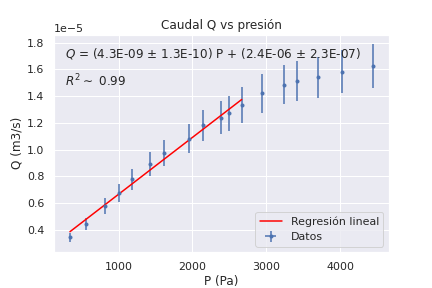
\includegraphics[width=\linewidth]{caudal_vs_presion}
	\caption{Caudal volumétrico de agua en función de $\Delta p$}
	\label{figure_caudal}
\end{figure}

Hay que notar que la recta ajustada no pasa por el origen, sino que predice un caudal nulo para un valor negativo de $\Delta p$, por lo tanto debemos corregir el valor de $\Delta p$ para obtener una recta que efectivamente pase por el origen. En este sentido si identificamos la ecuación de la recta de la figura (\ref{figure_caudal}) tal que $0 = mP+b$ obtenemos un factor de corrección dado por $P' = \frac{b}{m}$. Dado que $\Delta p$ será transformado a $\Delta p'$, debemos tener en cuenta la propagación de errores de dicha transformación, es decir $\epsilon_{p'} = \epsilon_{p} + |\frac{\epsilon_{b}}{m}| + |\frac{b\epsilon_{m}}{m^2}|$. En la figura (\ref{figure_caudal_corregida}) vemos el nuevo ajuste lineal. En este caso comprobamos que se conserva el valor de la pendiente, que el término independiente es prácticamente cero y que los errores en el eje de presión se han incrementado.

\begin{figure}[t]
	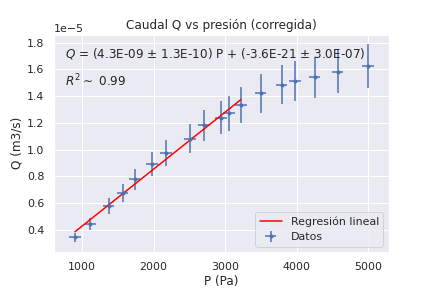
\includegraphics[width=\linewidth]{caudal_vs_presion_corregida}
	\caption{Caudal volumétrico de agua en función de $\Delta p'$ corregida}
	\label{figure_caudal_corregida}
\end{figure}

En términos generales vemos que el caudal es directamente proporcional a la presión en una región que identificamos con el flujo laminar del fluido, dado por el ajuste de mínimos cuadrados, hasta llegar a un punto de aparición de un codo, el cual representa el punto de transición hacia el régimen turbulento. La propagación de errores hace énfasis en este tramo (turbulento) de la dificultad de hallar un valor de caudal lo suficientemente certero.

Mediante la ley de Hagen-Poiseuille, ecuación (\ref{eq_caudal}), identificamos el factor $\frac{\pi r^4 \Delta p}{8\mu L}$ con la pendiente de la regresión lineal, de tal manera que $\mu = \frac{\pi r^4 \Delta p}{8\alpha L}$ donde $\alpha = (4.3 \pm 0.13)\cdot 10^{-9}m^3/Pa\cdot s$. Así pues obtenemos que la viscosidad dinámica es $\mu = (3.2 \pm 0.4) \cdot 10^{-3} Pa \cdot s$, valor que difiere notablemente de su análogo teórico $\mu_t = 0.001 Pa \cdot s$ a una temperatura de 20ºC, siendo el valor experimental tres veces mayor mayor que el valor teórico. Estas diferencias pueden deberse a una discordancia de temperaturas a la que se ha calculado la viscosidad, pues en nuestro caso el laboratorio se encontraba a 27ºC. Además, debido a la propia disposición del dispositivo experimental, no podemos garantizar la exactitud de los valores medidos (distancia, presión, tiempo), que sin un análisis de errores experimentales influye negativamente en los cálculos sucesivos. Por otro lado, la densidad del agua (ideal) para nuestros cálculos no corresponde no el agua utilizada en nuestro experimento.

A partir de estos datos experimentales y gracias a la ecuación (\ref{eq_reynolds}) podemos calcular el número de Reynolds (recordar que $U = \frac{Q}{\pi r^2}$). Los datos correspondientes los podemos ver en la tabla (\ref{table_exp}). Los datos inferiores a la línea horizontal central representan aquellos que corresponden al régimen laminar y con los que se llevó a cabo la regresión lineal (Q vs $\Delta p'$). 

Examinando los datos podemos confirmar el comportamiento $\Delta p \propto Q \propto U$, pues al aumentar la presión aumentará el caudal y, por consiguiente, la velocidad media del agua dentro del tubo capilar. Además comprobamos el régimen laminar para todos aquellos valores que, sumando su correspondiente incertidumbre, están dentro del límite $Re < 2000$. Sin embargo, aunque no obtenemos ningún valor para el número de Reynolds que esté por encima de dicho límite, sí reconocemos la transición al régimen turbulento para todos aquellos valores que sumando la incertidumbre están en el rango $2000<Re<3000$. Como hemos visto, obtenemos, en general, valores inferiores a los esperados con incertidumbres muy altas (sobretodo en régimen transitorio).

También podemos ver en la tabla (\ref{table_exp}) los valores calculados para el coeficiente de resistencia $\lambda$ según la ecuación (\ref{eq_lambda}) y (\ref{eq_lambda_reynolds}). Aunque dichos valores tienen una incertidumbre tal que solapan en rango unos con otros, es importante recalcar que tienen una incertidumbre muy alta (pues son función del número de Reynolds), tanto que el error relativo para este coeficiente está en el rango de entre 30\% y el 40\%, cumpliéndose el 30\% para todos los valores de $\lambda_{64}$. 

En la figura (\ref{figure_lambda}) hemos representado los datos para $\lambda$ en función de $Re$. Las líneas representan las soluciones a la ecuación (\ref{eq_karmann_prandtl}) característica del régimen turbulento. Se ha preferido graficar dichas líneas para el régimen laminar (donde no son válidas) para observar su comportamiento. Podemos identificar entonces que la solución de la ecuación trascendente que más se asemeja a nuestros datos es la línea (morada) que está justo por encima de nuestros puntos experimentales para los valores más altos del número de Reynolds.

Podemos hacer énfasis en el régimen turbulento mediante una presentación logarítmica de nuestros datos. En la figura (\ref{figure_lambda_log}) podemos ver el comportamiento lineal de $log (\lambda)$ frente a $log (Re)$ para el régimen laminar y su correspondiente punto de inflexión hacia el régimen turbulento, marcado por un cambio de tendencia con pendiente positiva.

\begin{figure}[t]
	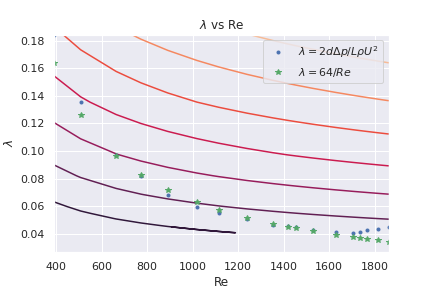
\includegraphics[width=\linewidth]{3lambda_nolog_noerror}
	\caption{Diagrama de Moody. Comportamiento del coeficiente de resistencia $\lambda$ según el número de Reynolds. Las líneas representan las soluciones a la ecuación (\ref{eq_karmann_prandtl}) de Karmann-Prandtl. No se incluyen barras de error debido a su gran tamaño.}
	\label{figure_lambda}
\end{figure}

\begin{figure}[t]
	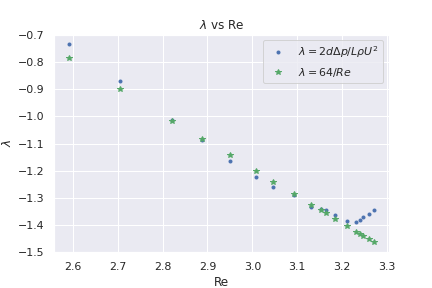
\includegraphics[width=\linewidth]{2lambda_log_noerror}
	\caption{Diagrama de Moody logarítmico para el coeficiente de resistencia. No se incluyen barras de error debido a su gran tamaño.}
	\label{figure_lambda_log}
\end{figure}